\documentclass[12pt,letterpaper]{article}

% ── Geometry ──────────────────────────────────────────────────────────
\usepackage[margin=1in,headheight=14pt]{geometry}

% ── Fonts (XeLaTeX) ──────────────────────────────────────────────────
\usepackage{fontspec}
\setmainfont{DejaVu Serif}

% ── Spacing ──────────────────────────────────────────────────────────
\usepackage{setspace}
\onehalfspacing
\usepackage{parskip}
\tolerance=1500
\emergencystretch=1em

% ── Math ─────────────────────────────────────────────────────────────
\usepackage{amsmath}
\usepackage{amssymb}

% ── Tables ───────────────────────────────────────────────────────────
\usepackage{booktabs}
\usepackage{array}

% ── Figures ──────────────────────────────────────────────────────────
\usepackage{graphicx}
\usepackage{float}

% ── Captions ─────────────────────────────────────────────────────────
\usepackage[font=small,labelfont=bf]{caption}

% ── Headers ──────────────────────────────────────────────────────────
\usepackage{fancyhdr}
\pagestyle{fancy}
\fancyhf{}
\fancyhead[L]{\small\itshape Pagadala}
\fancyhead[R]{\small\itshape Education of Humanity}
\fancyfoot[C]{\thepage}
\renewcommand{\headrulewidth}{0.4pt}

% ── Colors and hyperlinks ─────────────────────────────────────────────
\usepackage{xcolor}
\usepackage[colorlinks=true,linkcolor=blue!60!black,citecolor=blue!60!black,urlcolor=blue!60!black,
  pdftitle={Education of Humanity},
  pdfauthor={Krishna Pagadala}]{hyperref}

% ── Code / script references ─────────────────────────────────────────
\usepackage{listings}
\lstset{basicstyle=\small\ttfamily,breaklines=true}

% ── CSQuotes ─────────────────────────────────────────────────────────
\usepackage{csquotes}

% ── Section formatting ───────────────────────────────────────────────
\usepackage{titlesec}
\titleformat{\section}{\Large\bfseries}{\thesection.}{0.5em}{}
\titleformat{\subsection}{\large\bfseries}{\thesubsection}{0.5em}{}

% ══════════════════════════════════════════════════════════════════════
% DOCUMENT
% ══════════════════════════════════════════════════════════════════════

\begin{document}

% ── Title ─────────────────────────────────────────────────────────────
\begin{titlepage}
\begin{center}
\vspace*{3cm}
{\LARGE\bfseries Education of Humanity\par}
\vspace{2cm}
{\large Krishna Pagadala\par}
\vspace{0.5cm}
{\normalsize\itshape 2026\par}
\end{center}
\thispagestyle{empty}
\end{titlepage}

\setcounter{page}{2}

% ══════════════════════════════════════════════════════════════════════
% 1. WHAT HUMANS ARE
% ══════════════════════════════════════════════════════════════════════

\section{What Humans Are}

Education is fundamental to human well-being. Not important ---
fundamental. The distinction matters. Important means high on a list.
Fundamental means the list does not exist without it.

Every other species on earth reaches adult competence within months or
a few years. Humans take roughly eighteen. That is not a deficiency. It
is the mechanism. Eighteen years of sustained dependency --- the longest
juvenile period of any species --- creates something that exists nowhere
else in nature: a dedicated learner embedded with a dedicated teacher
for nearly two decades. Long enough for cumulative cultural knowledge to
be absorbed so deeply that it becomes the learner's own baseline. The
learner then becomes the teacher. The cycle has no natural end point.
What travels through this channel is cultural, not genetic. But the
channel itself is biological. It requires the species-specific
parent-child dependency period that only humans possess.

This is Parental Transmission: PT. The parent is the critical channel
--- the one that fires with biological certainty. But humans are a
social species. Siblings tutor younger siblings. Extended families in
multigenerational households transmit educational norms across shorter
intervals. Communities set expectations. Diaspora invest back in home
regions. The parent guarantees the floor. The society around the parent
determines how fast and how far the signal reaches. A parent transmits
to the child not just knowledge but norms, aspirations, health
behaviours, and the decision to send the next child to school. The
grandchild's attainment reflects the grandparent's through two
sequential cycles. The great-grandchild's through three. Education
compounds across generations because the channel that carries it is
built into the species --- and amplified by every social structure
humans build around it.

Formal schooling is the most powerful payload ever delivered through
this channel. The neuroscience is unambiguous: literacy physically
restructures the brain's visual processing pathways; numeracy recruits
parietal circuits unavailable to innumerate populations. These are not
marginal improvements on existing capacities. They are new cognitive
technologies that do not develop without schooling, regardless of
intelligence or environment. A stunted child who learns to read
undergoes the same categorical reorganisation as a well-nourished one.
The distance from no formal education to any formal education is
categorical. The distance from a bad school to a great school is
marginal by comparison.

PT fires on this categorical threshold. The household decision to send
a daughter to school, to space births, to recognise symptoms, to
vaccinate a child --- these are the decisions of educated adults
exercising agency across a lifetime. The approximately 25-year lag
between educational investment and development outcomes is not a
statistical artefact. It is the interval for educated children to become
adults and begin making these decisions. States can create conditions
for these decisions. They cannot make them.

PT explains why educational gains never depreciate. At no point in any
country's trajectory does educational attainment decline from one
generation to the next. The gains are irreversible because they are
embodied in people, not stored in budgets or institutions. Income can
be removed by economic crisis. Provision can be removed by fiscal
collapse. Both happen routinely. Education cannot be removed because it
lives in the teacher, not the institution. The only way to remove
education is to kill the educated. Cambodia tested this. The damage
lasted a generation.

The invisibility of this mechanism is itself a product of the mechanism.
Educated people consistently rate education as important --- one of many
important things, ranked alongside health, nutrition, governance, and
security. They cannot categorise it as fundamental, because that would
require seeing their own cognition from outside --- recognising that the
capacity to evaluate, compare, and advocate is itself the product of
education. The people who could identify education as fundamental are
inside it. The people who would benefit most from it are outside it.
The historical exceptions confirm the rule: John Knox acted from
religious conviction. Meiji Japan from existential military threat.
Korea from Cold War survival. In every case where the decisive
commitment was made, the motivation came from outside the development
frame entirely.


% ══════════════════════════════════════════════════════════════════════
% 2. THE PROOF
% ══════════════════════════════════════════════════════════════════════

\section{The Proof}

The claim is testable. If education is fundamental --- the input
without which no other mechanism operates --- then three things must be
true in the data. Education must predict development outcomes that
income does not. Education's predictive power must persist across
multiple generations while income's fades. And once education is
removed from income, income must have nothing left to predict.

All three are confirmed across 187 countries and 140 years of data.

\subsection{Education predicts. Income does not.}

In 187-country panel data with country fixed effects --- isolating
within-country variation over time --- one generation's education
predicts the next generation's development outcomes 25 years later.

Each one percentage point gain in lower secondary completion predicts,
one generation forward: 1.2\% higher GDP per capita, 0.108 more years
of life, and 0.032 fewer children per woman. These are identified from
within-country variation after controlling for initial conditions.

Among the countries where the expansion is still active --- parental
completion below 30\%, where most of the remaining undeveloped 20\% of
humanity sits --- education leads income by 3.3 to 1 as a predictor of
the next generation's education. GDP's predictive power barely changes
across cutoffs. Education's jumps from 0.54 to 0.70. GDP has no
S-curve structure. Education does.

The asymmetry sharpens when the outcome is life expectancy. Among
countries below 30\% completion, education predicts life expectancy one
generation forward at R\textsuperscript{2}=0.309. GDP predicts it at
R\textsuperscript{2}=0.021 --- education leads by 15 to 1.

\subsection{Education persists. Income fades.}

Measured across lag lengths from 0 to 100 years, education and income
have structurally different decay profiles. Education's predictive
power for life expectancy decays slowly across three generational
depths: R\textsuperscript{2}=0.562 at lag 0,
R\textsuperscript{2}=0.364 at lag 25, R\textsuperscript{2}=0.171 at
lag 50, R\textsuperscript{2}=0.085 at lag 75. Income collapses within
one generation --- already fading by lag 20--25. Beyond lag 50, income
data does not thin out. It was uniformly low. Every pre-literate
subsistence society sat at approximately \$400--600 per capita. Income
had no cross-country variation because education had not yet created it.

In human terms: in countries that were still expanding, a
great-grandparent's completion predicts how long their
great-grandchild will live --- four generations later. No other
development input has a comparable reach.

\subsection{Remove education from income, and income predicts nothing.}

The comparison above overstates income's role, because education drives
GDP growth --- countries develop serially, education rises first, income
follows a generation later. To isolate GDP's independent predictive
power, I residualize GDP against education within countries and use the
residual --- the component of GDP not explained by education --- to
predict each development outcome one generation forward.

The result is unambiguous across every outcome tested:

\begin{figure}[H]
\centering
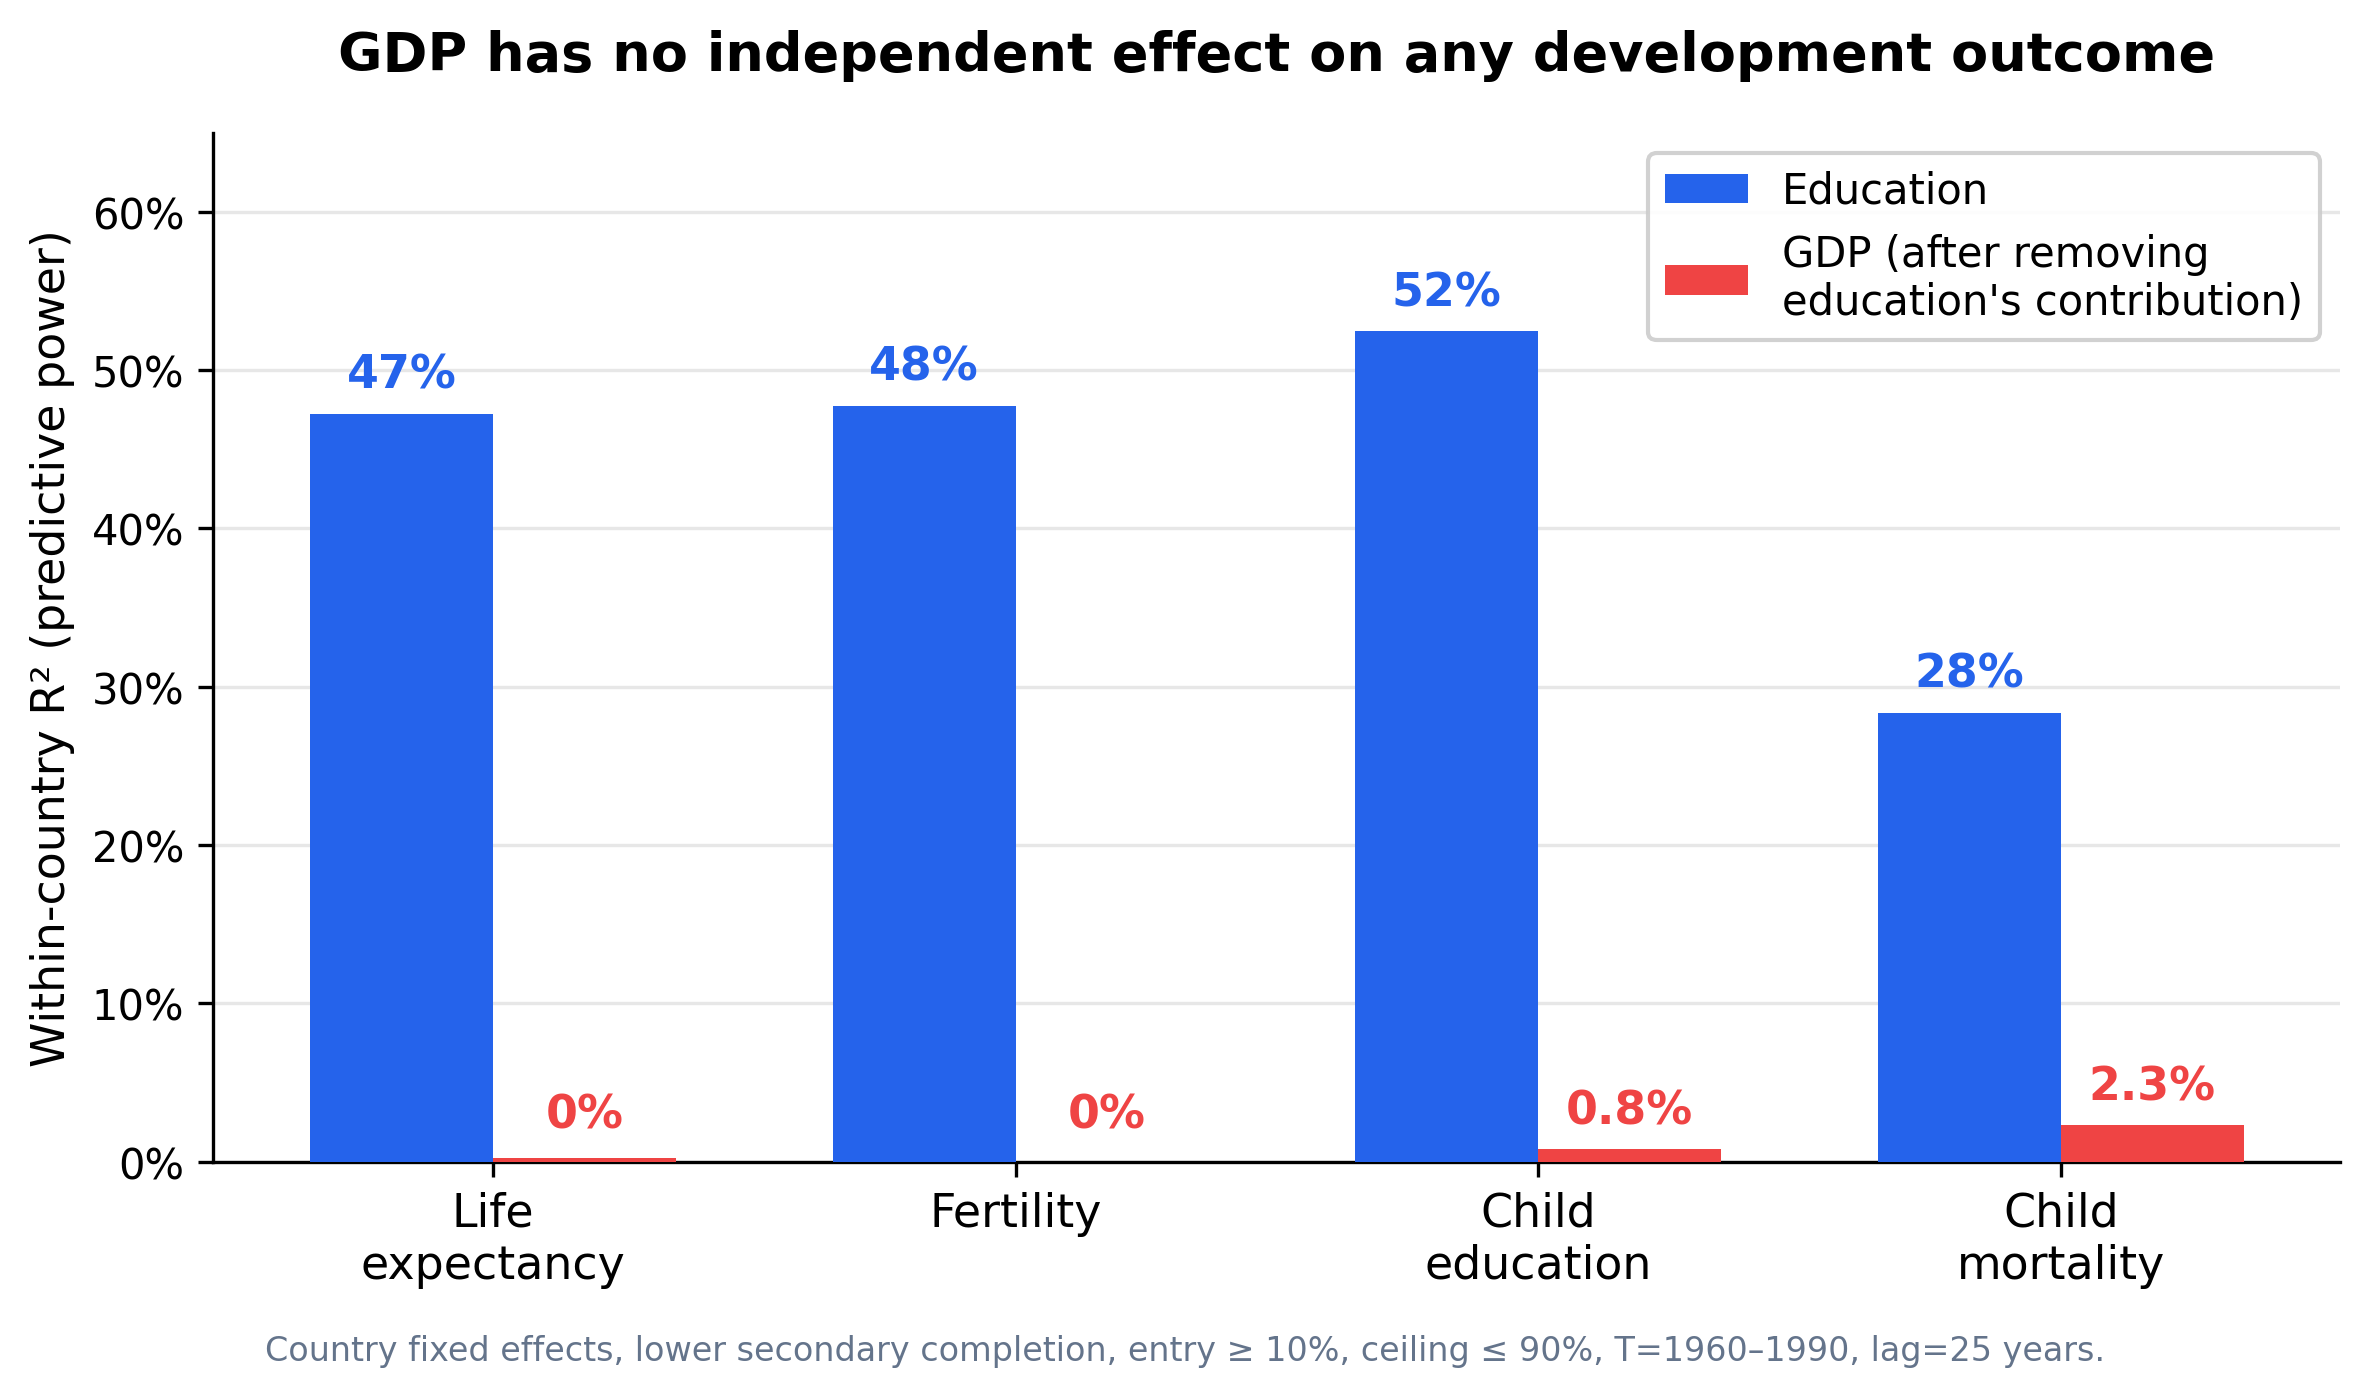
\includegraphics[width=\textwidth]{fig_residualization.png}
\caption{Education R\textsuperscript{2} vs.\ residualized GDP
R\textsuperscript{2} across four development outcomes. Blue: education
predicting each outcome one generation forward. Red: GDP after removing
education's contribution. Country fixed effects, entry-cohort design,
lag=25 years. \emph{(Source: author's calculation. See
\texttt{scripts/fig\_residualization.py})}}
\label{fig:residualization}
\end{figure}

After removing education's contribution to GDP, income has no
independent predictive power for any development outcome. The
residualized GDP R\textsuperscript{2} never exceeds 0.023. The
associated p-values are all above 0.1 --- statistically
indistinguishable from zero. Education explains 42\% of within-country
GDP variation; the remaining 58\% of GDP predicts nothing about the
future.

GDP appeared to matter only because education was flowing through it.
The mechanism is education, not income.


% ══════════════════════════════════════════════════════════════════════
% 3. THE CASES
% ══════════════════════════════════════════════════════════════════════

\section{The Cases}

A country is developed when it has simultaneously achieved a total
fertility rate below 3.65 and life expectancy above 69.8 years --- the
1960 United States values. By 2022, 154 countries representing 80\% of
the world's population have crossed both thresholds. Every one through
education. The variation is only in speed.

\begin{figure}[H]
\centering
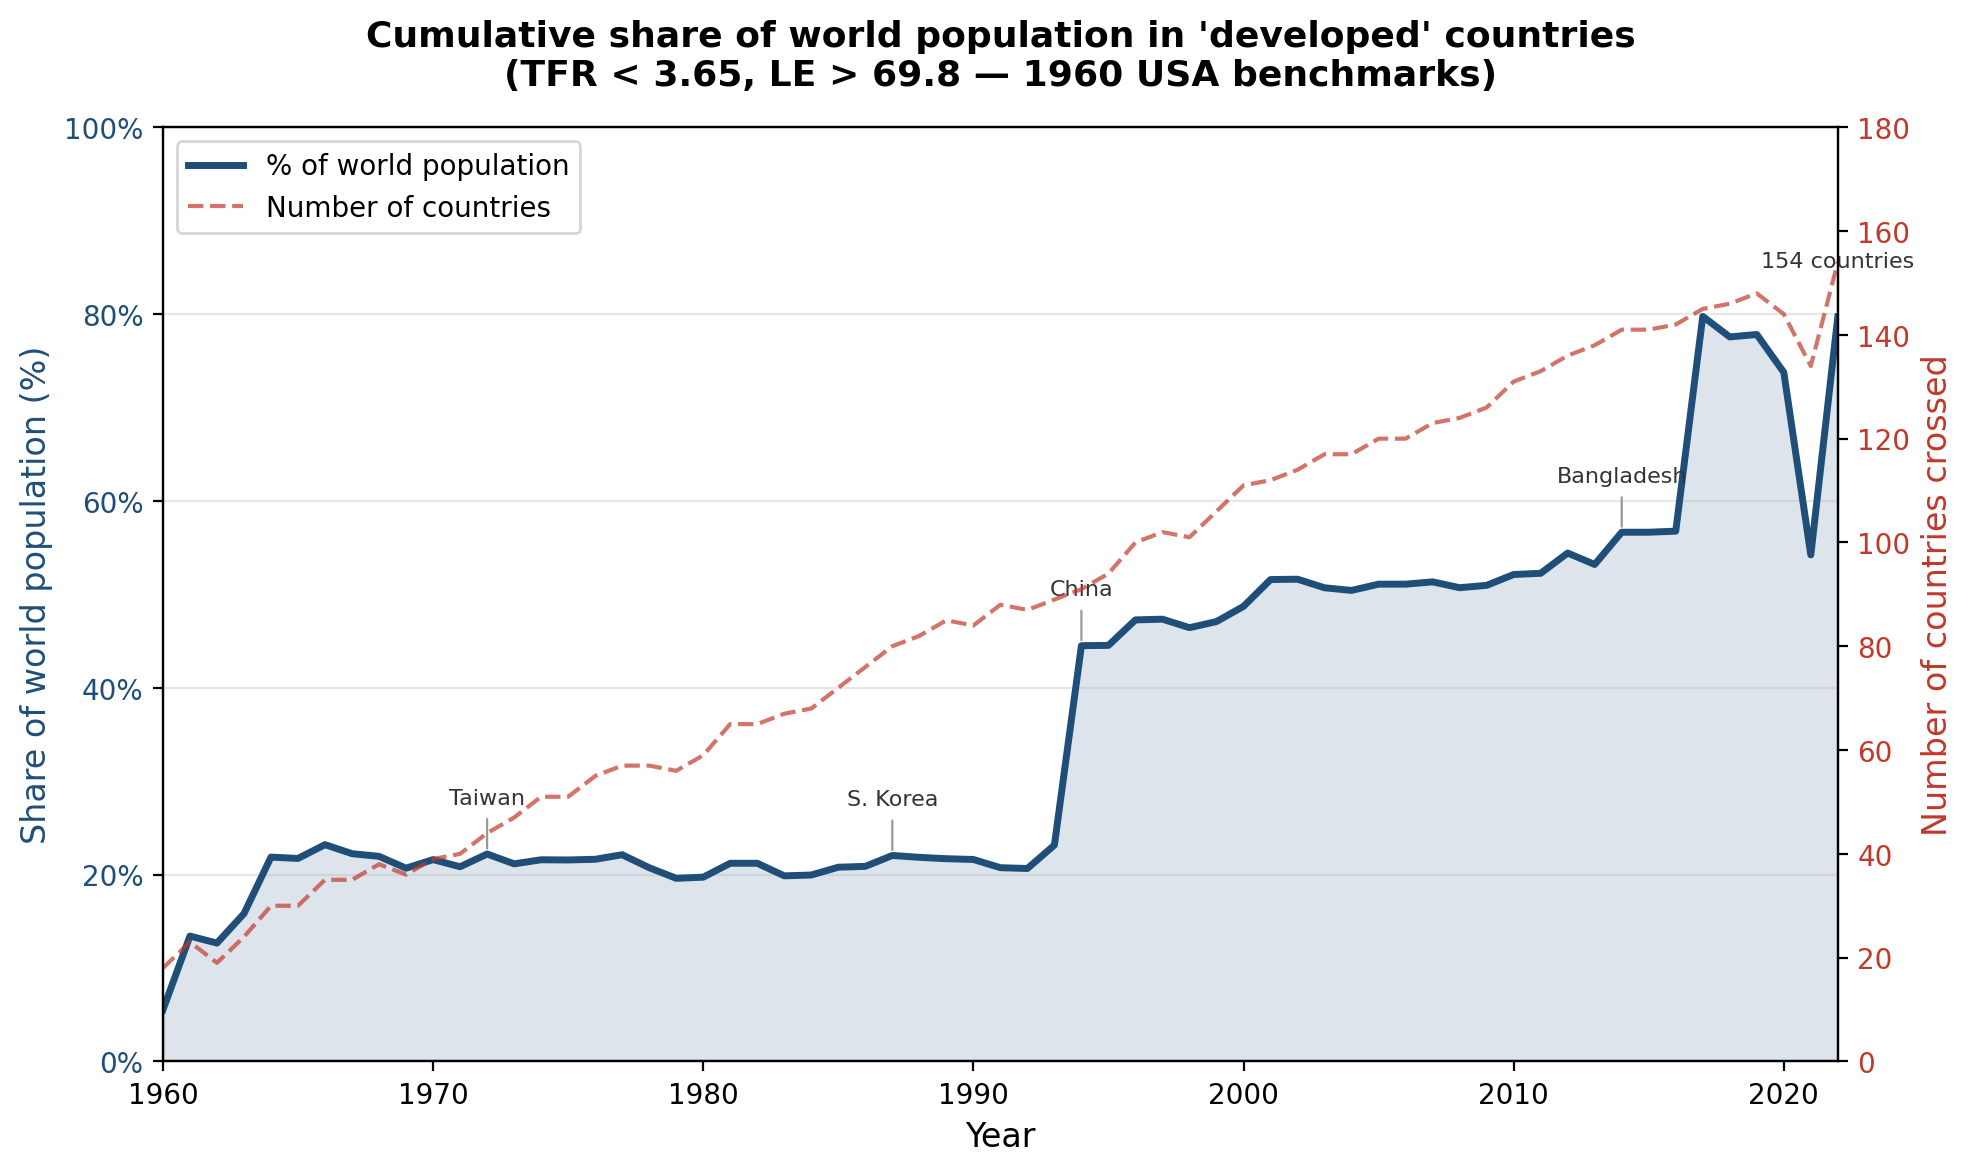
\includegraphics[width=\textwidth]{fig_cumulative_developed.png}
\caption{Cumulative share of world population crossing both
development thresholds, 1960--2022. \emph{(Source: World Bank WDI, WCDE v3.
See \texttt{scripts/fig\_cumulative\_developed.py})}}
\label{fig:cumulative}
\end{figure}

\begin{table}[H]
\centering
\caption{Year of development and relationship to prior education
investment. Thresholds are 1960 United States values (World Bank WDI).}
\label{tab:crossing}
\small
\begin{tabular}{lcccll}
\toprule
Country & Developed & TFR crossed & LE crossed & Expansion onset & Lag \\
\midrule
Taiwan & $\sim$1970 & $\sim$1970 & $\sim$1970 & 1950s & $\sim$20 yrs \\
S.\ Korea & 1987 & 1975 & 1987 & 1953--65 & $\sim$25 yrs \\
Cuba & 1974 & 1972 & 1974 & 1961 (40\% base) & $\sim$13 yrs \\
Bangladesh & 2014 & 1995 & 2014 & 1990s & $\sim$24 yrs \\
Sri Lanka & 1993 & 1981 & 1993 & 1940s--50s & $\sim$42 yrs \\
China & 1994 & 1975 & 1994 & 1950s+CR & $\sim$42 yrs \\
Uganda & --- & TFR 5.25 & LE 63.8 & None & --- \\
\bottomrule
\end{tabular}
\end{table}

\textbf{Korea: 35 years.} One of the poorest countries in the world in
1953. GDP per capita of \$1,038. Made education the unconditional
national priority. Expanded lower secondary completion from 25\% to
near-universal in 35 years --- 7 to 14 percentage points per five-year
period, sustained without interruption. Fertility fell and life
expectancy rose before Korea was rich. The mechanism did not wait for
income. By the time income arrived, the educated population converted
it into one of the world's largest economies. Korea's generational
transmission coefficient started at 6.5 at 1\% baseline and fell
steadily to 0.2 as completion approached 90\% --- the signature of
state investment amplifying what households transmit, then ceiling
compression as everyone is educated.

\textbf{Bangladesh: \$1,159.} The most important case in the table.
Lower secondary completion was 11.4\% in 1960. GDP per capita was
\$1,159 in 2014 when it crossed both development thresholds. The
premise that income is the prerequisite for development is directly
refuted. Bangladesh made the decision to treat girls' education as the
primary investment from the 1990s onward. The gender gap in children's
completion collapsed. TFR decline tracked girls' secondary expansion,
not contraceptive distribution. The LE and TFR gains came through
educated household decisions --- the same micro-decision pathway
visible in every case in this table. Bangladesh is already a policy
over-performer: +15.8 percentage points above its own generational
baseline. The over-performance was the sustained expansion. The 2014
crossing was its result, approximately 24 years later. Income is not
the mechanism.

\textbf{Cambodia: the PT shadow.} Cambodia shows what happens when
education is destroyed --- and how long the damage lasts. Under the
Khmer Rouge (1975--1979), the education system collapsed. Lower
secondary completion was 10.1\% in 1975. It fell to 9.4\% by 1980 and
was still at 9.5\% in 1985 --- a full decade of zero progress while the
rest of the world advanced. After reconstruction, completion jumped to
35\% by 1995. Then it stalled again. From 1995 to 2010, completion
plateaued at 31--36\% despite continued international investment. The
buildings were there. The teachers were there. The money was there.
Progress did not come. External supply could recover completion to the
pre-disruption parental baseline. It could not push beyond it without
the parental cohort catching up. The children reaching secondary school
in 1996--2010 were born approximately 1982--1996 --- their parents were
the cohort whose education was frozen at 10\% during 1975--1985.
Recovery began only after 2011, when the post-disruption cohort's
children entered the system. The twenty-year gap between the buildings
coming back (1991) and progress resuming (2011) is the PT shadow.
Vietnam, starting at 20\% in 1960, reached 81\% by 2015 without
interruption. Cambodia, on a similar trajectory, was at 36\%. The gap
is one generation of stalled parental education, expressing itself in
the educational attainment of the next.

\textbf{Spain: 450 years of wealth without development.} The richest
empire on earth for two hundred years. Spain controlled more gold and
silver than any nation in history. It did not develop until it finally
educated its people in the late twentieth century. Spain had 0.6\%
primary completion for the 1875 birth cohort. Universal lower secondary
completion arrived only in the 1970s. Development followed. Wealth was
never the mechanism. Britain took centuries. The United States and Japan
each took about a century. Korea did it in 35 years. The variable is
not wealth. It is the decision to educate.

\textbf{China: the largest educational expansion in history.} Three
corrections to the standard narrative. First, the TFR threshold was
crossed in 1975 --- five years before the one-child policy. The most
famous population policy in human history was unnecessary: the
threshold was already crossed before coercion began. Second, what is
universally called an educational catastrophe --- the Cultural
Revolution --- was in fact the largest lower secondary expansion in
China's WCDE record. For approximately 80\% of the population living in
rural China, community schools brought secondary education to villages
that had none. The base of the pyramid expanded dramatically while the
apex was disrupted. Third, the barefoot doctors and the community school teachers came
from the same CR-era rural mobilisation. The teachers mattered more.
When Deng dismantled the barefoot doctor network after 1980, China's
LE continued to rise --- from approximately 64 to 69.8 by 1994 ---
because the educational baseline built into rural households did not
leave with the doctors. The crossing dates follow mechanically from
starting distance, not from provision model.


% ══════════════════════════════════════════════════════════════════════
% 4. THE DECISION
% ══════════════════════════════════════════════════════════════════════

\section{The Decision}

154 countries representing 80\% of the world's population have already
crossed both development thresholds. Every one through education. No
country has developed without it. No country with sustained educational
expansion has failed to develop.

The remaining 20\% is concentrated in sub-Saharan Africa, with Pakistan,
Afghanistan, and Yemen as the largest exceptions outside the continent.
These populations are not facing an untested proposition. They are
facing a mechanism that has already delivered for four-fifths of the
world.

The question is not whether development will arrive through income
growth or state provision. That debate describes how resources flow
through different institutional channels --- markets or state services
--- not the underlying cause. Where educational expansion is fast and
markets function, income growth becomes visible and gets credited.
Where expansion is slow and markets are absent, state services are the
only observable welfare activity and they get credited instead. Both
are downstream of education. The taxonomy that dominates development
policy is a description of surface appearances, not causes.

The question is whether the decision is made. The decision is sustained
state commitment to expand education --- particularly girls' education
--- as the primary national objective, maintained across political
cycles and competing priorities.

The historical record maps onto three speeds. \textbf{Singular
priority}: the state makes education the unconditional national focus.
One-generation crossing. Korea, Taiwan, Cuba. \textbf{Competing
priority}: education competes with health, nutrition, security, and
governance for funding and political attention. Multi-generational. India
and most post-colonial countries. \textbf{PT alone}: without state
investment, a parent transmits what they have. The next generation does
the same. Century-scale, as in pre-modern Europe.

None of these required high income. Korea did it at \$1,038 per capita.
Bangladesh at \$1,159. Nepal at \$423 and 27\% completion is already a
policy over-performer at +17.8 percentage points above its generational
baseline. The mechanism does not care about regime type, ideology, or
income level. Korea, Taiwan, Cuba, and Bangladesh crossed under
authoritarian rule, democracy, socialism, and one of the poorest
economies on earth respectively. The mechanism cares whether the
decision is made.

Once made, the gains are irreversible --- embodied in people, not stored
in budgets --- and visible within a single political term: completion
rates rise within 5--10 years of sustained investment, providing the
metric a leader needs before the generational returns arrive. The only
way to remove education is to kill the people who carry it. Everything
else follows from the decision to educate, transmitting through PT into
every generation after.

The household mechanism that drives fertility decline, child survival,
and the next generation's schooling fires through mothers. Girls'
education is the highest-return lever in the entire system. Primary
education is the strongest predictor of fertility decline --- the
categorical jump from no schooling to literacy is where fertility falls
hardest. Life expectancy gains accumulate with deeper education. The
steepest demographic headwinds are at the lowest completion levels,
where population growth is rapid and the gains from each educated cohort
are diluted across a larger and faster-growing next generation.
Sustained state investment is required all the way to near-universal
completion. Korea's data shows steady expansion from 25\% to over 90\%
with no inflection at any point.

The 154 countries that have already crossed took between 13 and 450
years. The variation is explained entirely by when the decision was
made and whether it was sustained. A country that makes the decision
today, at Korea's pace, crosses the development threshold within 35
years. At half Korea's pace, within two generations.

Twenty years is enough to change the trajectory for every country that
has not yet crossed. The mechanism is not a theory. It has already
delivered for four-fifths of the world. The remaining fifth is not
waiting for income, institutions, or provision. It is waiting for the
decision.

\vspace{2em}

\section*{Data and Replication}

Education data: WCDE v3, lower secondary completion, both sexes, age
20--24. GDP: World Bank WDI, constant 2017 USD per capita. Life
expectancy, TFR, under-5 mortality: World Bank WDI. Development
thresholds: 1960 United States values (TFR = 3.65, LE = 69.8).

Panel: 187 countries, 1950--2015 at five-year intervals. Generational
panel: 1975--2015, 1,683 country-years. Long-run analysis: 28-country
subsample extending to 1900. All regressions use country fixed effects.
Parental education: each country's lower secondary completion lagged 25
years.

Full analysis code, data, and verification outputs available at\\
\href{https://github.com/rkpagadala/education-of-nations}%
{github.com/rkpagadala/education-of-nations}.

\section*{Acknowledgments}

All code and data analysis were produced by Claude (Anthropic), working
under the author's direction. Claude also assisted with prose drafting
and argument testing. The arguments, theories, and conclusions are
entirely the author's.

\end{document}
